\documentclass[tikz]{standalone}
% \usetikzlibrary{arrows.meta}
\usetikzlibrary{patterns.meta}
\begin{document}

	% [-latex, arrows={-Triangle[angle=20:5pt,scale=1.5]}]
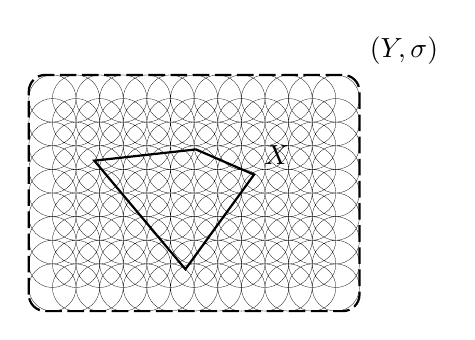
\begin{tikzpicture}[scale=0.6]
	\draw [thick,dash pattern = on 6pt off 2pt, rounded corners=6pt] 
	(0,0) rectangle (7,5) node [above right] {\((Y, \sigma)\)};
	\draw [ultra thin] \foreach \n in {1,...,9} \foreach \m in {1,...,13} 
	{(\m/2,\n/2) circle (0.5cm)};
	\begin{scope}[shift={(3.5,3)}]
		\draw [thick, rotate=-50, scale=3] 
		(-0.5,-0.5) -- (-0.1,0.1) -- (0.3,0.3) node [above right] {\(X\)}
		-- (0.5,-0.5) -- cycle;
	\end{scope}
\end{tikzpicture}

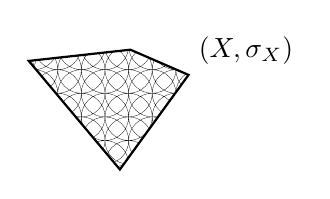
\begin{tikzpicture}[scale=0.6,shift={(3.5,3)}]
		\draw [thick, rotate=-50, scale=3] 
		(-0.5,-0.5) -- (-0.1,0.1) -- (0.3,0.3) node [above right] {\((X, \sigma _X)\)}
		-- (0.5,-0.5) -- cycle;
		\clip [rotate=-50, scale=3] 
		(-0.5,-0.5) -- (-0.1,0.1) -- (0.3,0.3) -- (0.5,-0.5) -- cycle;
		\begin{scope}[shift={(-3.5,-3)}]
	\draw [ultra thin] \foreach \n in {1,...,9} \foreach \m in {1,...,13} 
	{(\m/2,\n/2) circle (0.5cm)};
		\end{scope}
\end{tikzpicture}
\end{document}
